\documentclass[11pt,fleqn]{article}
\usepackage{../cs70,graphicx, latexsym,epsf, amssymb, framed}


% Space between paragraphs
\setlength{\parskip}{10pt plus 1pt minus 1pt}

\lecture{5}
\def\title{Note \the\lecturenumber}

\newcounter{thm}
\addtocounter{thm}{\the\lecturenumber}

\newtheorem{theorem}{Theorem}[thm]
\newtheorem{algorithm}{Algorithm}[thm]
\newtheorem{lemma}{Lemma}[thm]
\newtheorem{fact}{Fact}[thm]
\newtheorem{definition}{Definition}[thm]
\newtheorem{conjecture}{Conjecture}[thm]
\newtheorem{counterexample}{Counterexample}[thm]
\newtheorem{corollary}{Corollary}[thm]
\newtheorem{observation}{Observation}[thm]

\begin{document}
\maketitle


\section{The Stable Marriage Problem}\label{scn:intro}

In the previous note, we discussed the powerful proof technique of induction. In this note, we apply induction to analyze the solution to an important problem known as the \emph{Stable Marriage Problem}, which we now introduce.

Suppose you run a dating agency, and your task is to match up $n$ men and $n$ women. Each man has an ordered {\it preference list\/} of the $n$ women,
and each woman has a similar list of the $n$ men. 
For example, consider the case of $n=3$, i.e. three men Alex, Bob, and Charles, and three women Anita, Bridget, and Christine, with the following preference lists (lists are ordered from most favorable to least favorable):
\begin{center}
    \begin{tabular}{|c|c|}
      \hline
          \text{Men} & \text{Women} \\ \hline
      Alex & Anita \hspace{0.5cm} Bridget \hspace{0.5cm} Christine \\ \hline
      Bob & Bridget \hspace{0.5cm} Anita \hspace{0.5cm} Christine \\ \hline
      Charles & Anita \hspace{0.5cm} Bridget \hspace{0.5cm} Christine \\
      \hline
    \end{tabular}
\hspace{18mm}
    \begin{tabular}{|c|c|}
      \hline
          \text{Women} & \text{Men} \\ \hline
      Anita & Bob \hspace{0.5cm} Alex \hspace{0.5cm} Charles \\ \hline
      Bridget & Alex \hspace{0.5cm} Bob \hspace{0.5cm} Charles \\ \hline
      Christine & Alex \hspace{0.5cm} Bob \hspace{0.5cm} Charles \\
      \hline
    \end{tabular}
\end{center}
What you would like to do as head of the dating agency is to pair up each man with a woman. For example, two possible pairings are \{(Alex, Anita), (Bob, Bridget), (Charles, Christine)\} and \{(Alex, Bridget), (Bob, Christine), (Charles, Anita)\}. However, you don't want just any old pairing! In order for your dating firm to be successful, you wish the pairing to make ``everyone happy'', in that nobody can realistically hope to benefit by switching partners. Can you do this efficiently?

It turns out that there is indeed an algorithm to achieve this; moreover, it's remarkably simple, fast, and widely-used. It's called the \emph{Stable Marriage algorithm} (a.k.a. the Gale-Shapley algorithm), and we present it now.

\section{The Stable Marriage Algorithm}\label{scn:alg}

\begin{framed}
  \noindent
  {\bf Every Morning:} Each man proposes to the most preferred woman on his list who has not yet rejected him.

  \noindent
  {\bf Every Afternoon:} Each woman collects all the proposals she received in the morning; to the man she likes best, she responds ``maybe, come back tomorrow'' (she now has him {\it on a string\/}), and to the others, she says ``never''.

  \noindent
  {\bf Every Evening:} Each rejected man crosses off the woman who rejected him
  from his list.

  The above loop is repeated each successive day until each woman has a man on a string; on this day, each woman marries the man she has on a string.
\end{framed}

Let's digest the algorithm by running it on our example above. The following table shows which men propose to
which women on the given day (the men in bold are ``on a string''):

\begin{center}
\begin{tabular}{|c|c|c|c|}
  \hline
  Days & Women & Proposals \\
  \hline
  1 & Anita & \textbf{Alex}, Charles \\
  &Bridget&\textbf{Bob}\\
  &Christine&---\\
  \hline
  2 & Anita & \textbf{Alex}\\
  &Bridget&\textbf{Bob}, Charles\\
  &Christine&---\\
  \hline
  3 & Anita & \textbf{Alex}\\
  &Bridget&\textbf{Bob}\\
  &Christine&\textbf{Charles}\\
  \hline
\end{tabular}
\end{center}
\noindent Thus, the algorithm outputs the stable pairing:
\{(Alex, Anita), (Bob, Bridget), (Charles, Christine)\}.

Before analyzing the algorithm's properties further, let's take a moment to ask one of the first questions you should always ask when confronted with a new concept: Why study stable marriage in the first place? What makes it and its solution so interesting? For this, we discuss the very real impact of the Gale-Shapley algorithm on the \emph{Residency Match} program.

\section{The Residency Match}\label{scn:residency}
Perhaps the most well-known application of the Stable Marriage
Algorithm is the residency match program, which pairs medical school
graduates and residency slots (internships) at teaching hospitals.
Graduates and hospitals submit their ordered preference lists,
and the stable pairing produced by a computer matches students
with residency programs.

The road to the residency match program was long and
twisted. Medical residency programs were first introduced
about a century ago. Since interns offered a source of cheap
labor for hospitals, soon the number of residency slots exceeded
the number of medical graduates, resulting in fierce competition.
Hospitals tried to outdo each other by making their residency
offers earlier and earlier. By the mid-40s, offers for residency
were being made by the beginning of junior year of medical school,
and some hospitals were contemplating even earlier offers ---
to sophomores! The American Medical Association finally stepped
in and prohibited medical schools from releasing student
transcripts and reference letters until their senior year.
This sparked a new problem, with hospitals now making ``short fuse"
offers to make sure that if their offer was rejected they could
still find alternate interns to fill the slot. Once again the
competition between hospitals led to an unacceptable situation,
with students being given only a few hours to decide whether
they would accept an offer.

Finally, in the early 1950's, this unsustainable situation led to the
centralized system called the National Residency Matching Program
(N.R.M.P.) in which the hospitals ranked the
residents and the residents ranked the hospitals. The N.R.M.P. then
produced a pairing between the applicants and the hospitals, though
at first this pairing was not stable.
It was not until 1952 that the N.R.M.P. switched
to the Stable Marriage Algorithm, resulting in a
stable pairing.

Finally, if the above still hasn't convinced you of the worth of this algorithm, consider this: In 2012, Lloyd Shapley and Alvin Roth won the Nobel Prize in
Economic Sciences by extending the Stable Marriage Algorithm\footnote{See \url{http://www.nobelprize.org/nobel_prizes/economic-sciences/laureates/2012/popular-economicsciences2012.pdf}
for details.}! (The moral of the story? Computer science pays off.)

\section{Properties of the Stable Marriage Algorithm}\label{scn:properties}

There are two properties we wish to show about the stable marriage algorithm: First, that it doesn't run forever, i.e. it halts, and second, that it outputs a ``good'' pairing. The former is easy to show; let us do it now.

\begin{lemma}\label{l:halts}
    The stable marriage algorithm halts.
\end{lemma}
\begin{proof}
    The argument is simple: On each day that the algorithm does not halt, at least one man must eliminate some woman from his list (otherwise the halting condition for the algorithm would be invoked). Since each list has $n$ elements, and there are $n$ lists, this means that the algorithm must terminate in at most $n^2$ days.
\end{proof}

Next, we'd like to show that the algorithm finds a ``good'' pairing. Before we do so, let's clarify what we mean by ``good''.

\subsection{Stability}\label{sscn:stability}
What properties should a good pairing have? Perhaps we'd like to maximize the number of
first ranked choices? Alternatively, we could minimize the number of last ranked choices. Or maybe it would be ideal to minimize the sum of the ranks of the choices, which may be thought of as maximizing the average happiness.

In this lecture we will focus on a very basic criterion:
\emph{stability}. A pairing is \textbf{unstable} if there is a man and a woman
who prefer each other to their current partners. We will call such a
pair a {\it rogue couple}. So a
pairing of $n$ men and $n$ women is \textbf{stable} if it has no rogue couples. Let us now recall our example from earlier:

\begin{center}
    \begin{tabular}{|c|c|}
      \hline
          \text{Men} & \text{Women} \\ \hline
      Alex & Anita \hspace{0.5cm} Bridget \hspace{0.5cm} Christine \\ \hline
      Bob & Bridget \hspace{0.5cm} Anita \hspace{0.5cm} Christine \\ \hline
      Charles & Anita \hspace{0.5cm} Bridget \hspace{0.5cm} Christine \\
      \hline
    \end{tabular}
\hspace{18mm}
    \begin{tabular}{|c|c|}
      \hline
          \text{Women} & \text{Men} \\ \hline
      Anita & Bob \hspace{0.5cm} Alex \hspace{0.5cm} Charles \\ \hline
      Bridget & Alex \hspace{0.5cm} Bob \hspace{0.5cm} Charles \\ \hline
      Christine & Alex \hspace{0.5cm} Bob \hspace{0.5cm} Charles \\
      \hline
    \end{tabular}
\end{center}

\sanity{Consider the following pairing for the example above: \{(Alex, Christine), (Bob, Bridget), (Charles, Anita)\}. Why is this pairing unstable? (Hint: Alex and Bridget are a rogue couple --- why?)}

Here is a stable pairing for our example: \{(Bob, Anita), (Alex, Bridget), (Charles, Christine)\}. Why is (Alex, Anita) \emph{not} a rogue couple here? It's certainly true that Alex would rather be with Anita than his current partner. Unfortunately for him, Anita would rather be with her current partner than with Alex. Note also that both Charles and Christine are paired with their \emph{least} favorite choice in this matching. Nevertheless, it \emph{is} a stable pairing, since none of their preferred choices would rather be with them.

Before we discuss how to find a stable pairing, let us ask a more basic question:
Do stable pairings always exist? Surely the answer is yes, since we could start
with any pairing and make it more and more stable as follows: If there is a rogue
couple, modify the current pairing so that they are together. Repeat. Surely this
procedure must result in a stable pairing? Unfortunately this reasoning is not sound! Why? Although pairing up the rogue couple reduces the number of rogue couples by one, it may also \emph{create new} rogue couples.

Let's further illustrate the fallacy of the reasoning above by applying it to a closely related scenario known as the \emph{Roommates Problem}. In this problem, we have $2n$ people who must be paired up to be
roommates (the difference being that unlike in stable marriage,
a person can be paired with any of the other $2n-1$ people, i.e. there is no concept of \emph{gender}). Now, suppose our approach of iteratively matching up rogue couples indeed \emph{did} work. Since this approach does not exploit the existence of different genders, we can apply it to the roommates problem. Thus, we conclude there must always exist a stable pairing for roommates. Wouldn't you be surprised then to read the following counterexample, which gives an instance of the roommates problem which does \emph{not} have a stable pairing!
\begin{center}
\begin{tabular}{|c|c|}
\hline
\multicolumn{2}{|c|}{\text{Roommates}} \\ \hline
A & B \hspace{0.5cm} C \hspace{0.5cm} D \\ \hline
B & C \hspace{0.5cm} A \hspace{0.5cm} D \\ \hline
C & A \hspace{0.5cm} B \hspace{0.5cm} D \\ \hline
D & -- \hspace{0.5cm} -- \hspace{0.5cm} -- \\
\hline
\end{tabular}
\end{center}%
We claim that in this instance, there always exists a rogue couple for any pairing. For example, the pairing \{(A,B), (C,D)\}
contains the rogue couple B and C. How about \{(B,C), (A,D)\}? This pairing is unstable because now A and C are a rogue couple.

\sanity{Verify that in this example there is {\it no\/} stable pairing!}

We conclude that any proof that there always exists a stable pairing in the stable marriage problem \emph{must} use the fact that there are two genders
in an essential way. In the next section we give such a proof, and a nifty one at that: We prove that there must exist a stable pairing because the stable marriage algorithm always outputs one!

\subsection{Analysis}\label{sscn:analysis}

We now prove that the stable marriage algorithm always outputs a stable pairing. Why should this be the case? Consider the following intuitive observation:

\begin{observation}\label{obs:worsebetter}
    Each man begins in the algorithm with his first choice being a possibility; as the algorithm proceeds, however, his best available option can only get \emph{worse} over time. In contrast, women's options can only get \emph{better} with time.
\end{observation}

Thus, as the algorithm progresses, each man's options get worse, while each woman's improves; at some point, the men and the women must ``meet'' in the middle, and intuitively such a pairing should be stable.

Let us formalize this intuition beginning with a formal statement of Observation~\ref{obs:worsebetter} via the following lemma.

\begin{lemma}[Improvement Lemma]\label{l:improve}
If man $M$ proposes to woman $W$ on the $k$th day, then on every subsequent day $W$ has someone on a string whom she likes at least as much as $M$.
\end{lemma}
\begin{proof}
We proceed by induction on the day $j$, such that $j\geq k$.

\emph{Base case $(j=k)$}: On day $k$, two cases are possible: (1) Either $W$ has nobody on a string, in which case she says ``maybe'' to $M$, or (2) she has another man $M'$ on a string, in which case, she says ``maybe'' to $M$ only if she prefers $M$ to $M'$. In either case, on day $k$, $W$ has someone on a string who she likes at least as much as $M$.

\emph{Inductive Hypothesis}: Suppose the claim is true for $j\geq k$.

\emph{Inductive Step}: We prove the claim for day $j+1$. By the Induction Hypothesis, on day $j$, $W$ had a man $M'$ on a string which she likes at least as much as $M$. On day $j+1$, two cases are possible: (1) Either nobody proposes to $W$, in which case $W$ keeps $M'$ on a string, or (2) a man $M''$ proposes to $W$, in which case, she says maybe to $M''$ only if she prefers $M''$ to $M'$. In either case, $W$ has someone on a string who she likes at least as much as $M$.
\end{proof}

\paragraph{Detour: The Well-Ordering Princple.} Let's take a moment to consider an alternate proof of Lemma~\ref{l:improve}; in the process, we'll uncover a fundamental principle which is equivalent to induction.

\begin{proof}[Alternate proof of Lemma~\ref{l:improve}]
As in our original proof, the claim certainly holds on day $j=k$. Suppose now, for sake of contradiction, that the $j$th
day for $j > k$ is the first counterexample where $W$ has either nobody
or some $M^\ast$ inferior to $M$ on a string. On day
$j - 1$, she has $M'$ on a string and likes $M'$ at least much as $M$.
According to the algorithm,
$M'$ still proposes to $W$ on the $j$th day since she said ``maybe'' the
previous day. So $W$ has the choice of at least one man on
the $j$th day; moreover, her best choice is at least as good as $M'$,
and according to the algorithm she will choose him over $M^\ast$. This contradicts
our initial assumption.
\end{proof}

What proof technique did we use to prove this lemma? Is it contradiction? Or some other beast entirely? It turns out that this \emph{also} a proof by induction! Why? Well, we began by establishing the base case of $j=k$. Next, instead of proving that for all $j$, $P(j)\lra P(j+1)$, we showed that the \emph{negation} of this statement is false, i.e. that ``there exists $j$ such that  $\neg(P(j)\lra P(j+1))$'' does not hold; thus, by the principle of the excluded middle, it must indeed hold that for all $j$, $P(j)\lra P(j+1)$!

\sanity{Ensure you understand why these two proofs are equivalent.}

Let us now be a bit more careful --- what exactly allowed us to take this alternate approach?
The answer lies in a very special property of the natural numbers known as the \emph{Well-Ordering Principle}. This principle intuitively says that any set of natural numbers contains a ``smallest'' element. Formally:
\begin{definition}[Well-ordering principle]
    If $S \subseteq \N$ and $S \neq \emptyset$, then $S$ has a smallest element.
\end{definition}

\sanity{Consider set $S=\set{5,2,11,7,8}\subset \N$. Verify that the well-ordering principle holds for $S$.}

Where did we use the well-ordering principle in our proof? In the line ``Suppose \ldots that the $j$th
day for $j > k$ is the first counterexample\ldots'' --- specifically, if the natural numbers did not obey this principle, then the notion of a \emph{first} counterexample would be nonsense! Note also that induction relies on this principle: The statement ``for all $j$, $P(j)\lra P(j+1)$'' only makes sense if there is a well-defined order imposed on the natural numbers (i.e. that $3$ comes before $4$, and $4$ comes before $5$, etc\ldots). That the natural numbers obey this principle may be a fact you have long taken for granted; but there do exist sets of numbers which do \emph{not} satisfy this property! In this sense, the natural numbers are indeed quite special.
\sanity{Do the integers satisfy the well-ordering principle? Can you think of a set of numbers you are familiar with which \emph{doesn't} satisfy this principle? (Hint: This set is as ``real'' as it gets.)}

\paragraph{Returning to our analysis of the stable marriage algorithm.} Returning to our analysis, we now prove that when the algorithm terminates, all
$2n$ people are paired up.
Before reading the proof, see if you can convince yourself that
this is true. The proof is remarkably short and elegant, and
critically uses the Improvement Lemma.

\begin{lemma}\label{l:pairing}
    The stable marriage algorithm terminates with a pairing.
\end{lemma}
\begin{proof}
We proceed by contradiction. Suppose that there is a man $M$ who is left
unpaired when the algorithm terminates. He must
have proposed to all $n$ of the women on his list. By the Improvement Lemma,
each of these $n$ women has had
someone on a string since $M$ proposed to her. Thus, when the algorithm terminates,
$n$ women have $n$ men on a
string not including $M$. So there must be at least
$n+1$ men. But this is a contradiction, since there are only $n$ men.
\end{proof}

Now, before we prove that the output of the algorithm is a \emph{stable} pairing,
let us first do a sample run-through
of the stable marriage algorithm. We will use the preference lists given
earlier, which are duplicated here for
convenience:
\begin{center}
    \begin{tabular}{|c|c|}
      \hline
          \text{Men} & \text{Women} \\ \hline
      Alex & Anita \hspace{0.5cm} Bridget \hspace{0.5cm} Christine \\ \hline
      Bob & Bridget \hspace{0.5cm} Anita \hspace{0.5cm} Christine \\ \hline
      Charles & Anita \hspace{0.5cm} Bridget \hspace{0.5cm} Christine \\
      \hline
    \end{tabular}
\hspace{18mm}
    \begin{tabular}{|c|c|}
      \hline
          \text{Women} & \text{Men} \\ \hline
      Anita & Bob \hspace{0.5cm} Alex \hspace{0.5cm} Charles \\ \hline
      Bridget & Alex \hspace{0.5cm} Bob \hspace{0.5cm} Charles \\ \hline
      Christine & Alex \hspace{0.5cm} Bob \hspace{0.5cm} Charles \\
      \hline
    \end{tabular}
\end{center}

\noindent The following table shows which men propose to
which women on the given
day (the circled men are the ones who were told ``maybe''):

\begin{center}
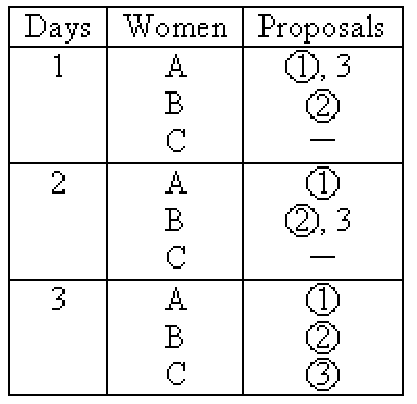
\includegraphics[scale = 0.7]{newstable}
\end{center}

\noindent Thus, the stable pairing which the algorithm outputs is:
\{(1,A), (2,B), (3,C)\}.

\begin{theorem}\label{thm:stable}
    The pairing produced by the algorithm is always stable.
\end{theorem}
\begin{proof}
We give a direct proof that no man $M$ can be involved in a rogue couple.
Consider any couple ($M$,$W$) in the
pairing and suppose that $M$ prefers some woman $W^\ast$ to $W$.
We will argue that $W^\ast$ prefers her partner to $M$, so that
($M$,$W^\ast$) cannot be a rogue couple. Since $W^\ast$
occurs before $W$ in $M$'s list, he must have proposed to her before he
proposed to $W$. Therefore, according
to the algorithm, $W^\ast$ must have rejected him for somebody she
prefers.
By the Improvement Lemma, $W^\ast$ likes her final partner at least as
much, and therefore prefers him to $M$.
Thus no man $M$ can be involved in a rogue couple, and the pairing is
stable.
\end{proof}

\section{Optimality}\label{scn:optimality}

In Section~\ref{sscn:analysis}, we showed that the stable marriage algorithm always outputs a stable pairing. But is this so impressive? Will your dating service really be successful outputting matches which are just ``good enough''? Of course not! To offer the best dating service around, you require some notion of \emph{optimality} in the solutions you obtain.

Consider, for example, the case of $4$ men and $4$ women with the
following preference lists (for simplicity, we use numbers and letters below to label the men and women):
\begin{center}
    \begin{tabular}{|c|c|}
      \hline
          \text{Men} & \text{Women} \\ \hline
      1 & A \hspace{0.5cm} B \hspace{0.5cm} C \hspace{0.5cm} D \\ \hline
      2 & A \hspace{0.5cm} D \hspace{0.5cm} C \hspace{0.5cm} B \\ \hline
      3 & A \hspace{0.5cm} C \hspace{0.5cm} B \hspace{0.5cm} D \\ \hline
      4 & A \hspace{0.5cm} B \hspace{0.5cm} C \hspace{0.5cm} D \\
      \hline
    \end{tabular}
\hspace{20mm}
    \begin{tabular}{|c|c|}
          \hline
          \text{Women} & \text{Men} \\ \hline
      A & 1 \hspace{0.5cm} 3 \hspace{0.5cm} 2 \hspace{0.5cm} 4 \\ \hline
      B & 4 \hspace{0.5cm} 3 \hspace{0.5cm} 2 \hspace{0.5cm} 1 \\ \hline
      C & 2 \hspace{0.5cm} 3 \hspace{0.5cm} 1 \hspace{0.5cm} 4 \\ \hline
      D & 3 \hspace{0.5cm} 4 \hspace{0.5cm} 2 \hspace{0.5cm} 1 \\
      \hline
    \end{tabular}
\end{center}

\noindent For these lists, there are exactly two stable
pairings: $S = $ \{(1,A), (2,D), (3,C), (4,B)\} and $T
= $ \{(1,A), (2,C), (3,D), (4,B)\}. The fact that there are \emph{two} stable pairings raises the question: What is the
best possible partner for each person? For example, let us consider man~$2$. The trivial best partner for $2$ is his first choice, woman $A$; unfortunately, $A$ is just not a realistic possibility for him, as pairing him with $A$ would not be stable, since he
is so low on her preference list. Indeed, there is no
stable pairing in which 2 is paired with~A. Examining the two stable pairings,
we find that the best possible realistic outcome for man~2
is to be matched to woman~D. This demonstrates that the notion of ``best partner'' can be a bit fuzzy if we are not careful.

So, let us be careful; inspired by the discussion above, here is a rigorous definition of optimality.

\begin{definition}[Optimal woman for a man]
Among all stable pairings, who is the most preferred woman a man can be paired up with? This woman is the \emph{optimal} woman for this man.
\end{definition}
In other words, the optimal woman is the best that a man can do in a pairing, given that the pairing is {stable}.

\sanity{Who are the optimal women for each man $A$, $B$, $C$, and $D$ in our example above? (Hint: The optimal woman for man $2$, as discussed above, is $D$.)}

By definition, the best that each man can hope for is to be paired with his
optimal woman. But can all men achieve this optimality {\it simultaneously\/}?
In other words, is there a stable pairing such that
each man is paired with his optimal woman? If such a pairing exists, we
will call it a {\it male optimal\/} pairing. Turning to the example above, $S$ is
a male optimal pairing since $A$ is $1$'s optimal woman, $D$ is $2$'s optimal
woman, $C$ is $3$'s optimal woman, and $B$ is $4$'s optimal woman. Similarly, we
can define a female optimal pairing, which is the pairing in which each
woman is paired with her optimal man.

\sanity{Check that $T$ is a female optimal pairing.}

We can also
go in the opposite direction and define the {\it pessimal\/} woman for
a man to be the lowest ranked woman whom he is ever paired with
in some stable pairing. This leads naturally to the notion of a {\it male
pessimal\/} pairing --- can you define it, and also a female pessimal
pairing?

Now, we get to the heart of the matter: Who is better off in the Stable Marriage Algorithm --- men or women?

\begin{theorem}\label{thm:maleopt}
    The pairing output by the Stable Marriage algorithm is male optimal.
\end{theorem}
\begin{proof}
Suppose for sake of contradiction that the pairing is {\it not\/} male optimal. Then, there exists a day on which some man was rejected by his optimal woman; let day $k$ be the first such day. On this day, suppose
$M$ was rejected by $W^*$ (his optimal mate) in favor of $M^*$. By definition
of optimal woman, there must be exist a stable pairing $T$ in which $M$ and $W^*$ are paired together.
Suppose $T$ looks like this: $\{\ldots,(M,W^*),\ldots,(M^*,W'),\ldots\}$.
We will argue that $(M^*,W^*)$ is a rogue couple in $T$, thus
contradicting stability.

First, it is clear that $W^*$ prefers $M^*$ to $M$, since she rejected $M$ in favor of $M^*$ during the execution of the stable marriage algorithm. Moreover, since day $k$ was the first day when some man got rejected by his optimal woman, on day $k$ $M^*$ had not yet been rejected by his optimal woman. Since he proposed to $W^*$ on the $k$-th day, this implies that $M^*$ likes
$W^*$ at least as much as his optimal woman, and therefore at least as much as $W'$. Therefore,
$(M^*,W^*)$ form a rogue couple in $T$, and so $T$ is not stable. Thus, we have a contradiction, implying the pairing is male optimal.
\end{proof}

What proof techniques did we use to prove this Theorem~\ref{thm:maleopt}? Again, it is a proof by induction,
structured as an application of the well-ordering principle.\\

\sanity{Where did we use the well-ordering principle in the proof of Theorem~\ref{thm:maleopt}?}

\exercise{Can you rewrite the proof of Theorem~\ref{thm:maleopt} as a regular induction proof? (Hint: The proof is really showing by induction on $k$ the following statement: For every $k$, no man gets rejected
by his optimal woman on the $k$th day.)}

We conclude that men fare very well by following this algorithm. How about the women? The following theorem confirms the sad truth:

\begin{theorem} \label{thm:femalepes}
    If a pairing is male optimal, then it is also female pessimal.
\end{theorem}
\begin{proof}
We proceed by contradiction. Let $T = \{\ldots, (M, W), \ldots\}$ be the male optimal pairing
(which we know is output by the algorithm by Theorem~\ref{thm:maleopt}).
Suppose for the sake of contradiction that there exists a stable pairing $S =
\{\ldots, (M^\ast, W), \ldots, (M, W'), \ldots\}$
such that $M^\ast$ is lower on $W$'s list than $M$ (i.e., $M$ is not her pessimal man).
We will argue that $S$ cannot be stable by showing that $(M,W)$ is a
rogue couple in $S$.  By assumption, $W$
prefers $M$ to $M^\ast$ since $M^\ast$ is lower on her list. And $M$ prefers $W$ to his
partner $W'$ in $S$ because $W$ is his partner in the male optimal pairing~$T$.
Contradiction. Therefore, the male optimal pairing is female pessimal.
\end{proof}

In light of these findings, what does the stable marriage algorithm teach us? When it comes to relationships, it pays to make the first move!

Let us close with some final comments about the National Residency Matching Program. Until recently the stable marriage algorithm was run with the
hospitals doing the proposing, and so the pairings produced were hospital
optimal. In the nineties, the roles were reversed so that the medical
students were proposing to the hospitals. More recently, there were
other improvements made to the algorithm which the N.R.M.P. used. For
example, the pairing takes into account preferences for married
students for positions at the same or nearby hospitals.

\section{Further reading (optional)}
Though it was in use 10 years earlier, the propose-and-reject algorithm
was first properly analyzed by Gale and Shapley, in a famous paper
dating back to 1962 that still stands as one of the great achievements in
the analysis of algorithms.  The full reference is:

D.~Gale and L.S.~Shapley, ``College Admissions and the Stability of Marriage,''
{\it American Mathematical Monthly\/} {\bf 69} (1962), pp.~9--14.

Stable marriage and its numerous variants remains an active topic of research
in computer science.  Although it is by now 25 years old, the
following very readable book covers many of the interesting developments since
Gale and Shapley's algorithm:

D.~Gusfield and R.W.~Irving, {\it The Stable Marriage Problem: Structure and Algorithms},
MIT Press, 1989.

\end{document}
